%\VignettePackage{LewyBodies.SN.Proteomics.BottomUp.Pub}
%\VignetteIndexEntry{LCMS Data Analysis}
%\VignetteDepends{vp.misc, BiocStyle, Biobase, MSnbase, msmsTests, GOstats, ReactomePA, DOSE, graphite, KEGGREST, reshape2, ggplot2, org.Hs.eg.db}
%\VignetteKeywords{Documentation}
%\VignetteEngine{knitr::knitr}

\documentclass[11pt]{article}\usepackage[]{graphicx}\usepackage[usenames,dvipsnames]{color}
%% maxwidth is the original width if it is less than linewidth
%% otherwise use linewidth (to make sure the graphics do not exceed the margin)
\makeatletter
\def\maxwidth{ %
  \ifdim\Gin@nat@width>\linewidth
    \linewidth
  \else
    \Gin@nat@width
  \fi
}
\makeatother

\definecolor{fgcolor}{rgb}{0.345, 0.345, 0.345}
\newcommand{\hlnum}[1]{\textcolor[rgb]{0.686,0.059,0.569}{#1}}%
\newcommand{\hlstr}[1]{\textcolor[rgb]{0.192,0.494,0.8}{#1}}%
\newcommand{\hlcom}[1]{\textcolor[rgb]{0.678,0.584,0.686}{\textit{#1}}}%
\newcommand{\hlopt}[1]{\textcolor[rgb]{0,0,0}{#1}}%
\newcommand{\hlstd}[1]{\textcolor[rgb]{0.345,0.345,0.345}{#1}}%
\newcommand{\hlkwa}[1]{\textcolor[rgb]{0.161,0.373,0.58}{\textbf{#1}}}%
\newcommand{\hlkwb}[1]{\textcolor[rgb]{0.69,0.353,0.396}{#1}}%
\newcommand{\hlkwc}[1]{\textcolor[rgb]{0.333,0.667,0.333}{#1}}%
\newcommand{\hlkwd}[1]{\textcolor[rgb]{0.737,0.353,0.396}{\textbf{#1}}}%
\let\hlipl\hlkwb

\usepackage{framed}
\makeatletter
\newenvironment{kframe}{%
 \def\at@end@of@kframe{}%
 \ifinner\ifhmode%
  \def\at@end@of@kframe{\end{minipage}}%
  \begin{minipage}{\columnwidth}%
 \fi\fi%
 \def\FrameCommand##1{\hskip\@totalleftmargin \hskip-\fboxsep
 \colorbox{shadecolor}{##1}\hskip-\fboxsep
     % There is no \\@totalrightmargin, so:
     \hskip-\linewidth \hskip-\@totalleftmargin \hskip\columnwidth}%
 \MakeFramed {\advance\hsize-\width
   \@totalleftmargin\z@ \linewidth\hsize
   \@setminipage}}%
 {\par\unskip\endMakeFramed%
 \at@end@of@kframe}
\makeatother

\definecolor{shadecolor}{rgb}{.97, .97, .97}
\definecolor{messagecolor}{rgb}{0, 0, 0}
\definecolor{warningcolor}{rgb}{1, 0, 1}
\definecolor{errorcolor}{rgb}{1, 0, 0}
\newenvironment{knitrout}{}{} % an empty environment to be redefined in TeX

\usepackage{alltt}
\usepackage[authoryear,round]{natbib}
\usepackage{booktabs}
\usepackage{colortbl, xcolor}
\usepackage{rotating}
\usepackage{graphicx}
\usepackage{caption}
\usepackage{makecell}
\usepackage[T1]{fontenc}
\usepackage{tabularx}
\usepackage{subfloat}
\usepackage{longtable}
\usepackage{caption}
\usepackage{multirow}
\usepackage[labelfont=bf]{caption}

\captionsetup{labelfont=bf}

\renewcommand{\rothead}[2][60]{\makebox[9mm][c]{\rotatebox{#1}{\makecell[c]{#2}}}}

% handling figure captions
\captionsetup{labelfont=bf}
% \captionsetup{textfont={color=gray,it,bf}}
\captionsetup{textfont={color=darkgray}}
\captionsetup{labelformat=empty}
% \renewcommand{\figurename}{Supplementary Figure}
% \newcommand{\reff}[1]{\textbf{Supplementary Figure \ref{#1}}}
\newcommand{\reff}[1]{}
\definecolor{highlighter}{HTML}{FFF8E1}

\RequirePackage{/usr/local/lib/R/site-library/BiocStyle/resources/tex/Bioconductor}









%~~~~~~~~~~~~~~~~~~~~~~~~~~~~~~~~~~~~~~~~~~~~~~~~~~~~~~~~~~~~~~~~~~~~~~~~~~~~~~~

\bioctitle[Analysis report: Petyuk et al., 2020]{
   {\Large Executable Analysis Document Supporting:}\\
    \textbf{Proteomic Profiling of the Substantia Nigra 
            to Identify Determinants of Lewy Body Pathology 
            and Dopaminergic Neuronal Loss}\\
   {\Large Part II: LC-MS/MS Data Analysis} \\
   % {\Large Molecular Neurodegeneration (2020) 
   %       \href{http://dx.doi.org/10.1038/ncb2881}{doi:10.1038/ncb2881}
   % }\\
}



\RequirePackage{color}
\definecolor{BiocBlue}{RGB}{24,129,194}
\makeatletter
\renewcommand{\maketitle}{
   \renewcommand\Authfont{\Large\bfseries}
   \renewcommand\Affilfont{\normalsize\mdseries\upshape}
   \thispagestyle{empty}
   {\huge\color{BiocBlue}\@title\unskip\strut\par}
   \addvspace{-4ex}
   {\@author\unskip\strut\par}
   {\large\bfseries\@date\unskip\strut\par}
}
\makeatother


\usepackage[noblocks]{authblk}
\author[1]{Vladislav A. Petyuk}
\author[2,3]{Lei Yu}
\author[4]{Heather M. Brewer}
\author[1]{Geremy Clair}
\author[1]{Wei-Jun Qian}
\author[5,6]{Joshua M. Shulman}
\author[2,3]{David A. Bennett}
%
\affil[1]{Biological Sciences Division, Pacific Northwest National Laboratory, Richland, WA, USA}
\affil[2]{Rush Alzheimer's Disease Center, Rush University Medical Center, Chicago, IL, USA}
\affil[3]{Department of Neurological Sciences, Rush University Medical Center, Chicago, IL, USA}
\affil[4]{Enviromental and Molecular Sciences Laboratory, Pacific Northwest National Laboratory, Richland, WA, USA}
\affil[5]{Departments of Neurology, Molecular \& Human Genetics, and Neuroscience, Baylor College of Medicine, Houston, TX, USA}
\affil[6]{Jan and Dan Duncan Neurological Research Institute, Texas Children's Hospital, Houston, TX, USA}

\date{\today}

%~~~~~~~~~~~~~~~~~~~~~~~~~~~~~~~~~~~~~~~~~~~~~~~~~~~~~~~~~~~~~~~~~~~~~~~~~~~~~~~
\IfFileExists{upquote.sty}{\usepackage{upquote}}{}
\begin{document}
\maketitle
\tableofcontents























\section{Objective}
The ultimate goal of the project is to explore proteome changes associated
with the histopathological features of the Parkinson's disease:
Lewy bodies and \textit{Substantia nigra} neuronall loss. This is a new
perspective in analysis of Parkinson's disease etiology.  As opposed to
using clinical diagnosis for study design we rely on
molecular and cellular changes presumably preceeding the onset of Parkinson's
disease.




\section{PCA. Supplementary Figure 3}
PCA is a common approach to identify structure within the data. For example, 
it can help to identify and visualize the extend of the batch effects.
Columns of the 96-well plate were identified as a source of technical bias.
Thus it should be included into the follow-up statistical models.

\begin{figure}[h!]
\center
\begin{minipage}{0.7\textwidth}
\begin{knitrout}
\definecolor{shadecolor}{rgb}{0.969, 0.969, 0.969}\color{fgcolor}

{\centering 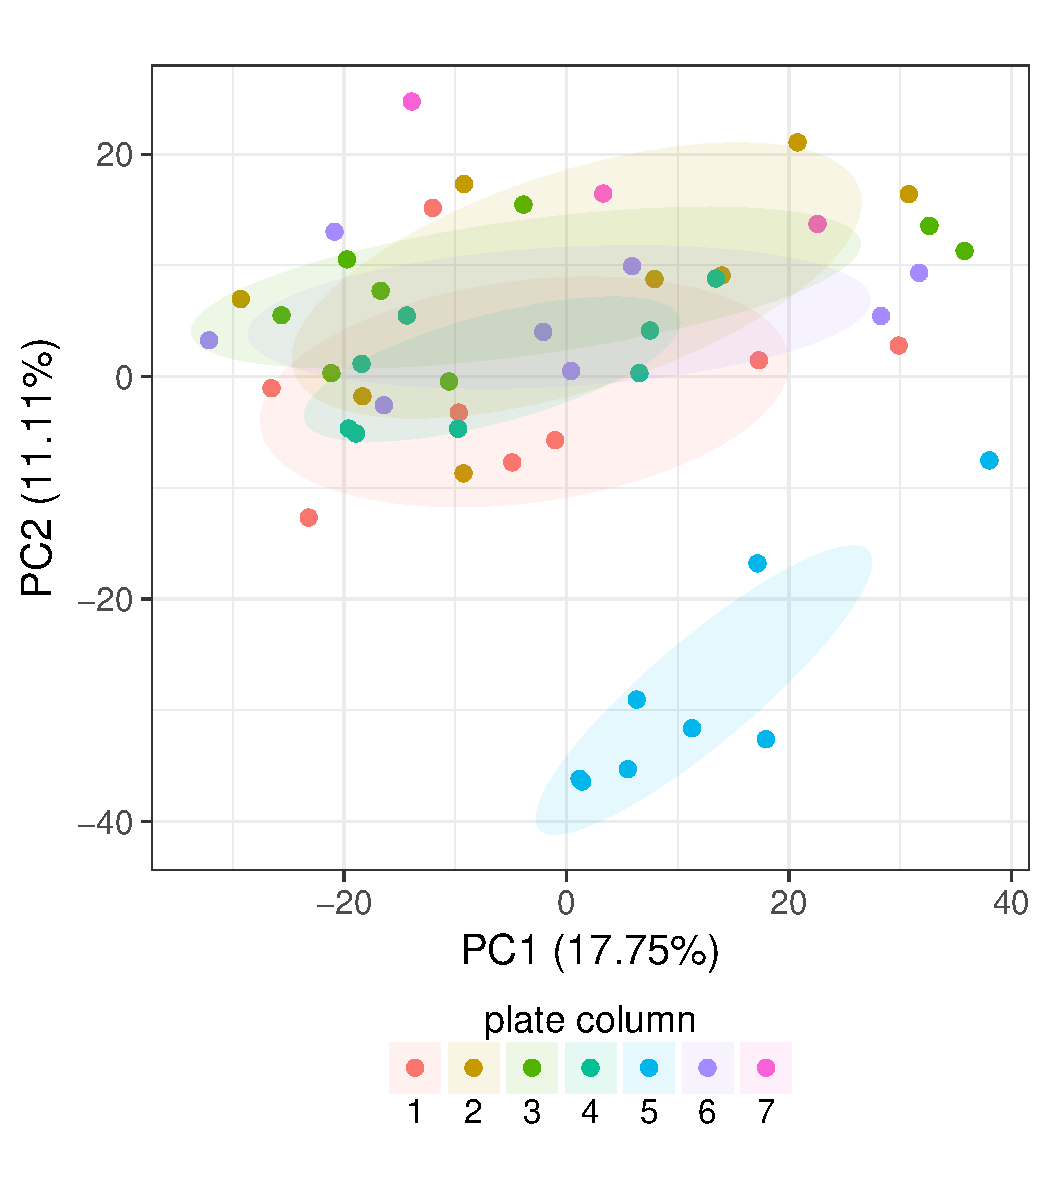
\includegraphics[width=0.6\textwidth]{figure/pca-1} 

}



\end{knitrout}
\caption{Corresponds to
\textcolor{black}{\colorbox{highlighter}{\textbf{Supplementary Figure 3}}}.
PCA plot of relative protein abundances. Samples colored according to the
column of the 96-well plate. The "batch" effect associated with the column
position is substantial to warrant it as a covariate in the statistical model.}
\label{fig:NLLBassoc}
\end{minipage}
\end{figure}

Percentage of proteins that statistically significantly affected by plate column effect.



\clearpage



% \section{Individual proteins. Figure 4}
% \begin{figure}[h!]
% \center
% \begin{minipage}{1\textwidth}
% <<individual_proteins,  out.width='1\\textwidth', fig.width = 16, fig.height = 8>>=
% 
% # data("SN_proteome_no_bias")
% load("SN_proteome_no_bias.RData")
% dSet <- cbind(pData(m), t(exprs(m)))
% 
% set.seed(0)
% trgts <- c('SNCA', 'TH', 'PARK7', 'VPS35', 'STK39', 'UCHL1', 'NPC1', 
%            'MCCC1', 'HIP1R', 'TMEM163', 'DLG2', 'VPS13C', 'BCKDK', 
%            'STX1B', 'DDRGK1', 'SCARB2', 'NUCKS1', 'GAK', 'APOE','SCARB2',
%            'ALDH1A1')
% 
% dSet2 <- dSet[,c('subject.type', trgts)]
% dSet2 <- gather(dSet2, key = protein, value = value, -subject.type)
% 
% g <- guide_legend(direction = "horizontal",
%                   nrow=1,
%                   title="subject type",
%                   title.hjust = 0.5,
%                   title.position = "top",
%                   title.theme = element_text(angle=0,size=18),
%                   label.position="bottom", 
%                   label.hjust = 0.5, 
%                   label.vjust = 0.5,
%                   label.theme = element_text(angle=0,size=16),
%                   keywidth = 6, keyheight = 2)
% 
% ggplot(dSet2, aes(x=subject.type, y=value, fill=subject.type)) +
%     geom_hline(yintercept = 0, col='#9E9E9E', size=0.5, linetype='dashed') +
%     geom_boxplot(aes(fill=subject.type), fill='white', outlier.shape = NA, size=0.3) +
%     geom_boxplot(aes(fill=subject.type), alpha=0.5, , outlier.shape = NA, size=0.3) +
%     geom_beeswarm(shape = 21, cex=4, size=2, stroke=0.5) +
%         # google logo colors
%         scale_fill_manual(values = c("case" = "#ea4335",
%                                  "control.1" =  "#ffeb3b",
%                                  "control.2" = "#34a853")) +
%     # ylab('log2 relative abundance') +
%     ylab(expression(protein~log[2]~relative~abundance)) +
%     xlab('subject type') +
%     # ylim(-1.5, +1.5) +
%     theme_bw(base_size = 18) +
%     theme(legend.position="none", 
%           axis.text.x=element_text(angle=90, hjust=1, vjust=0.5)) +
%     facet_wrap( ~ protein, scales = 'free_y', ncol = 7) +
%     guides(fill=g) +
%     theme(legend.position='bottom',
%           axis.ticks.x=element_blank(), 
%           axis.text.x=element_blank(), 
%           axis.text.y=element_text(size = 10), 
%           axis.title.x=element_blank(),
%           legend.direction = "horizontal",
%           legend.margin=unit(0.5,"cm"))
% ggsave(filename = 'Figure_4.png', width = 16, height = 8, scale = 1)
% @
% \caption{Corresponds to
% \textcolor{black}{\colorbox{highlighter}{\textbf{Figure 4}}} in the main text.
% Relative abundances of the selected proteins across the case/control groups. The proteins were selected based on significance in previous genetic, GWAS or PD biomarker studies. The relative abundances are adjusted for matching group effect and other confounding factors.}
% \label{fig:GObar}
% \end{minipage}
% \end{figure}



\clearpage



\section{Statistical significance analysis}
\subsection{Mixed effects model. Figure 3}
The protein abundances were modeled with linear mixed effects approach. 
The terms to consider are the subject type as 
fixed effect and matching group with 96-well plate column as random effects.
The full model in Wilkinson-Rogers notation is:
\begin{center}
$protein \sim subject.type + (1|PlateCol) + (1|match.group)$
\end{center}
The null model excludes the fixed subject type coefficient. The results of ANOVA
significance analysis are shown below.










\begin{figure}[h!]
\center
\begin{minipage}{1\textwidth}

\begin{knitrout}
\definecolor{shadecolor}{rgb}{0.969, 0.969, 0.969}\color{fgcolor}

{\centering 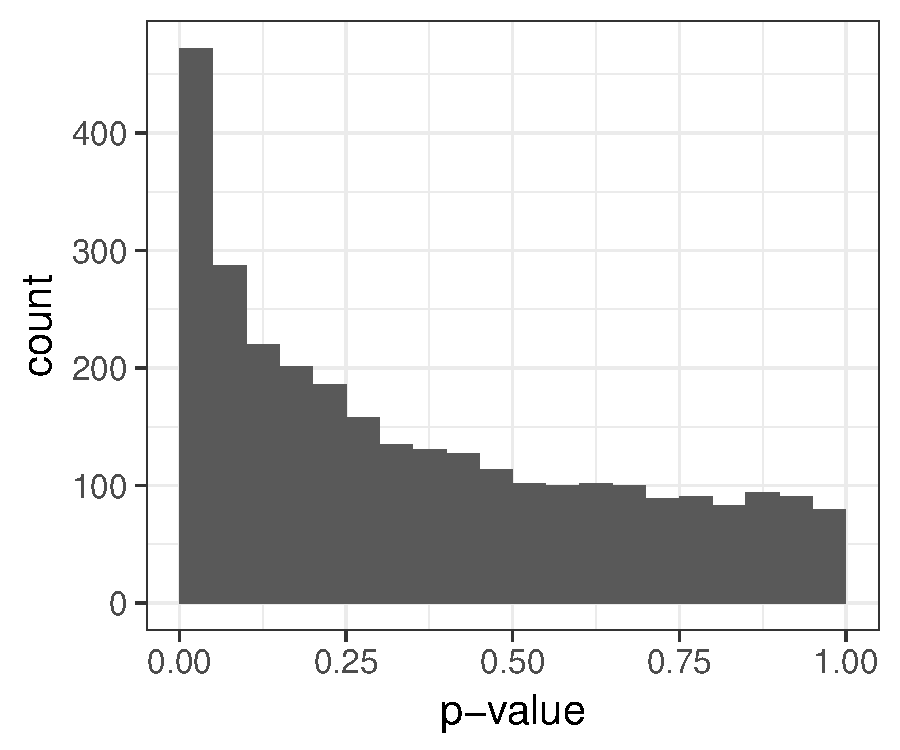
\includegraphics[width=0.5\textwidth]{figure/lmer_anova_test_results-1} 

}



\end{knitrout}

\caption{Corresponds to
\textcolor{black}{\colorbox{highlighter}{\textbf{Figure 3}}} in the main text.
P-value histogram of the mixed effects ANOVA test. Histogram bin width is 0.05. Higher then random number of proteins with low p-values (first bin) indicate on significance of the subject type effect.}
\label{fig:PValueHistogram}
\end{minipage}
\end{figure}

Full results of the ANOVA test available in the 
\textcolor{black}{\colorbox{highlighter}{\textbf{Supplementary Table 3}}}.













% latex table generated in R 3.3.2 by xtable 1.8-2 package
% Fri May  8 00:20:54 2020
\begin{table}[ht]
\centering
\begin{tabular}{lrrrrrr}
  \hline
{\bfseries  protein } & {\bfseries  p-value } & {\bfseries  q-value } & {\bfseries  adj. p-value } & {\bfseries  LB+NL+ } & {\bfseries  LB-NL+ } & {\bfseries  LB-NL- } \\ 
  \hline
RGS6 & 6.55e-05 & 0.11 & 0.19 & -0.14 & 0.11 & 0.03 \\ 
  EIF3E & 1.59e-04 & 0.13 & 0.24 & -0.08 & 0.18 & -0.10 \\ 
  CD59 & 2.54e-04 & 0.13 & 0.24 & 0.10 & -0.05 & -0.05 \\ 
  ITGB8 & 3.23e-04 & 0.13 & 0.24 & 0.02 & 0.22 & -0.24 \\ 
  PHYHIP & 4.64e-04 & 0.14 & 0.25 & 0.07 & -0.20 & 0.12 \\ 
  PSMA5 & 7.91e-04 & 0.14 & 0.25 & 0.10 & -0.07 & -0.03 \\ 
  PADI2 & 7.93e-04 & 0.14 & 0.25 & 0.09 & 0.12 & -0.21 \\ 
  OXSM & 8.42e-04 & 0.14 & 0.25 & -0.00 & -0.10 & 0.10 \\ 
  CLIC4 & 8.94e-04 & 0.14 & 0.25 & -0.00 & 0.20 & -0.19 \\ 
  CHDH & 9.03e-04 & 0.14 & 0.25 & 0.01 & 0.26 & -0.26 \\ 
   \hline
\end{tabular}
\caption{{\color{darkgray} Top 10 statistically significantly 
varying proteins across the subject types}} 
\end{table}




\subsection{Top 10 most significant proteins proteins. Figure 4}
\begin{figure}[h!]
\center
\begin{minipage}{1\textwidth}
\begin{knitrout}
\definecolor{shadecolor}{rgb}{0.969, 0.969, 0.969}\color{fgcolor}

{\centering 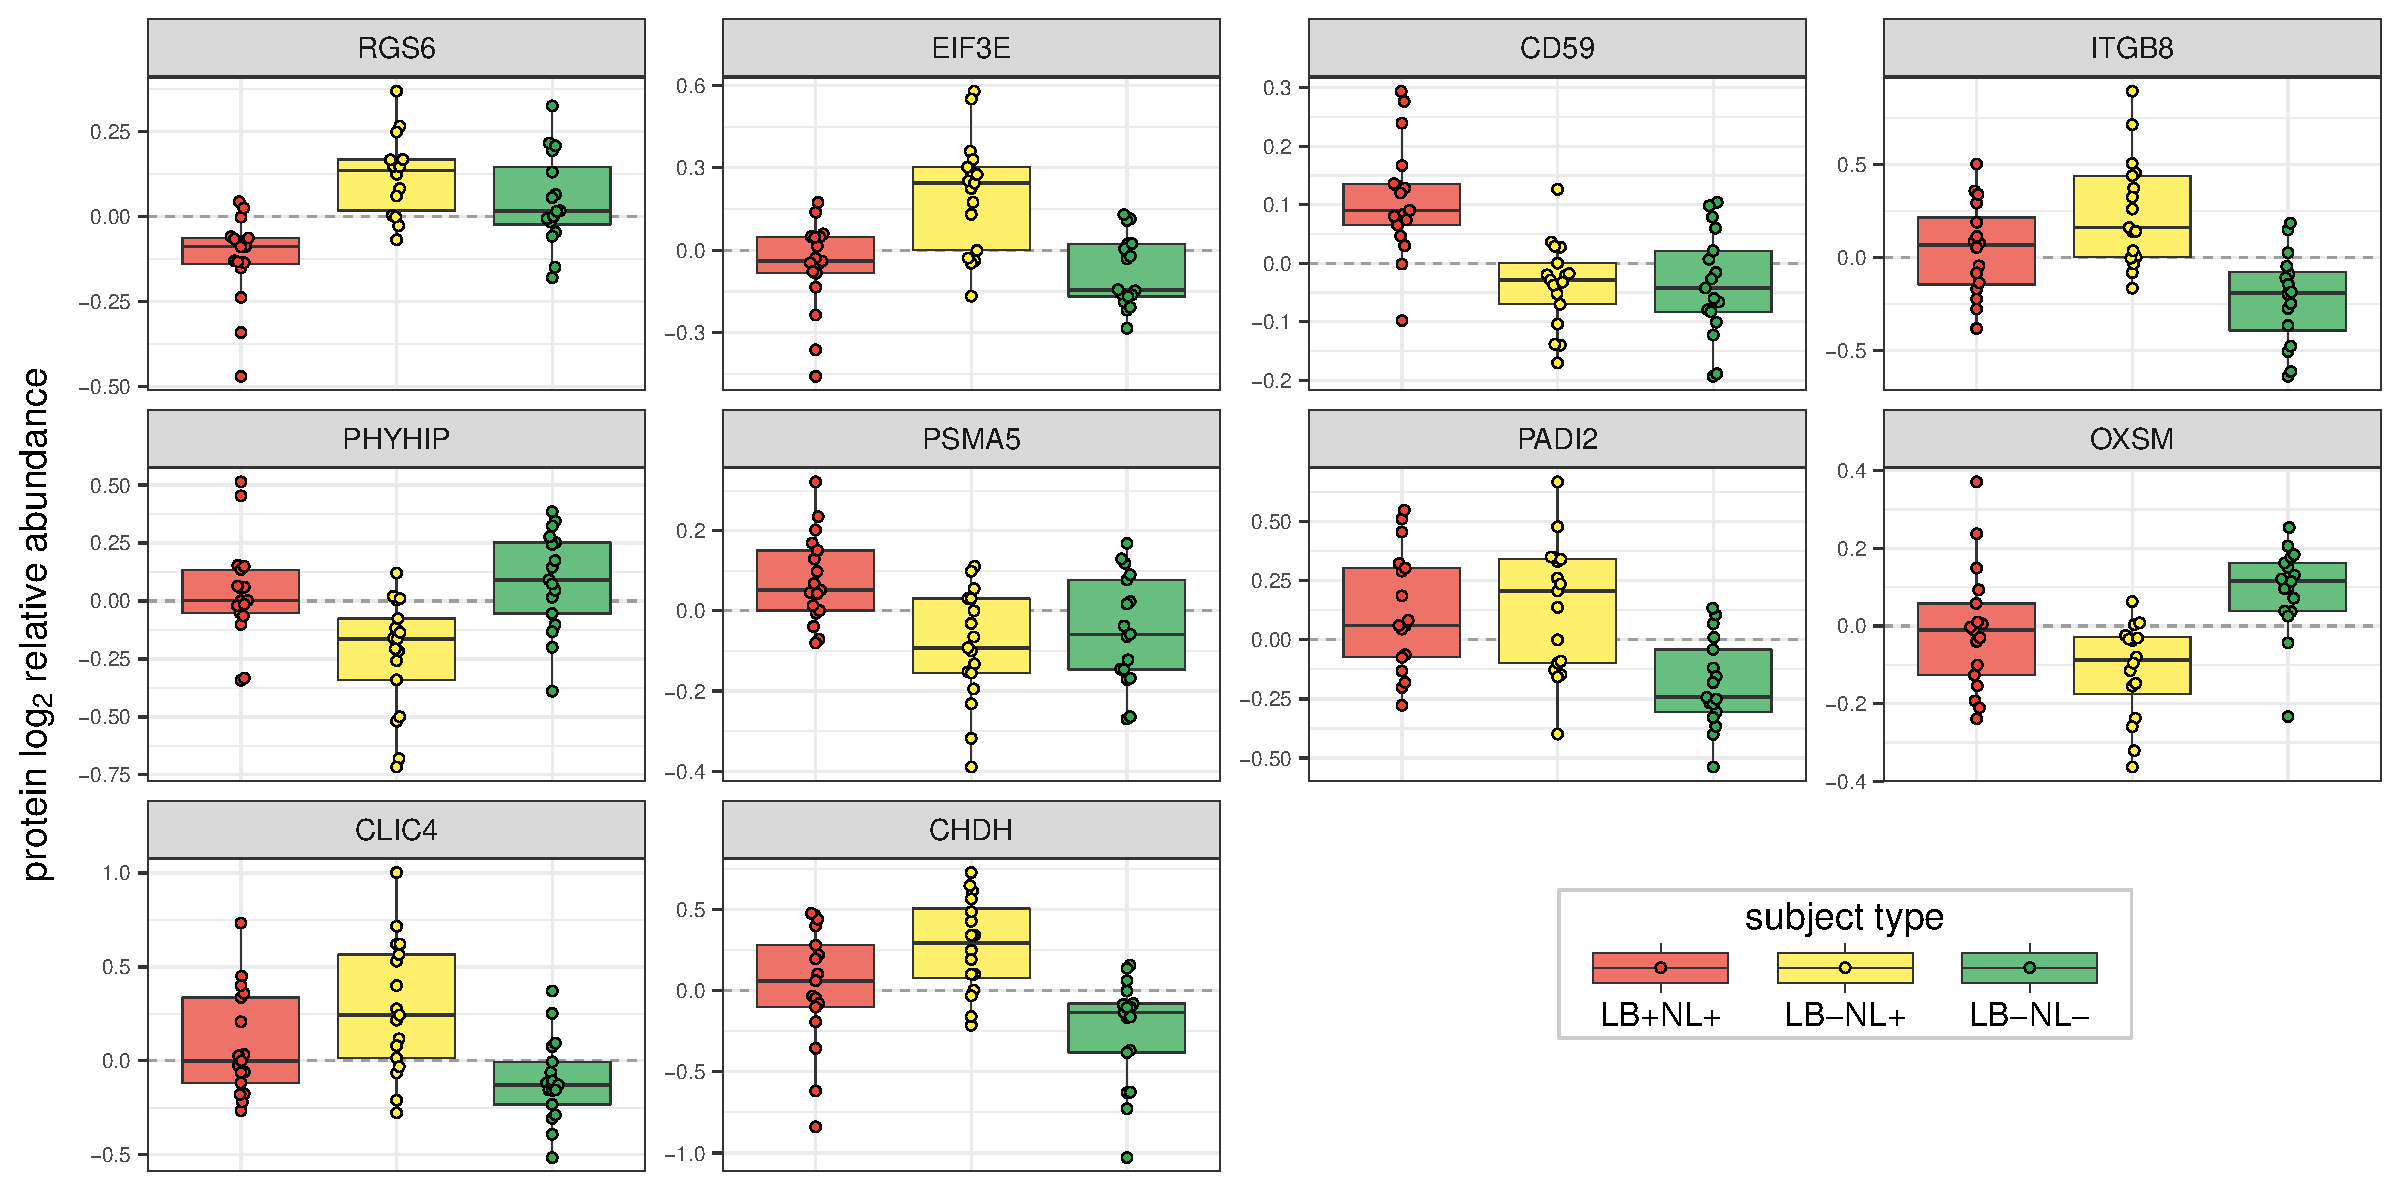
\includegraphics[width=1\textwidth]{figure/individual_proteins-1} 

}



\end{knitrout}
\caption{Corresponds to
\textcolor{black}{\colorbox{highlighter}{\textbf{Figure 4}}} in the main text.
Relative abundances of the top 10 most varying proteins across the groups. Proteins ordered according to significance in the ANOVA test. The relative abundances are adjusted for matching group effect and batch effect.}
\label{fig:Top10IndProt}
\end{minipage}
\end{figure}







\clearpage

\subsection{Top differential proteins for six contrasts. Table 2}
To obtain a detailed view on expression profiles acress the three subject types
we performed contrast analysis. The differential abundance was tested across six
contrasts including three pairwise comparisons and three comparisons of 
individual subject type vs the other two. Adjustment for multiplicity of 
comparisons was performed using single-step procedure based on z-statistic 
implemented in the \textbf{\Rcode{multcomp}} package.







{\centering
% latex table generated in R 3.3.2 by xtable 1.8-2 package
% Fri May  8 00:21:01 2020
\begin{table}[ht]
\centering
\begin{tabular}{llrr}
  \toprule
{\bfseries  contrast } & {\bfseries  protein } & {\bfseries  estimate } & {\bfseries  pvalue } \\ 
  \midrule
LB+NL+ vs LB-NL+ & RGS6 & -0.25 & 4.96e-06 \\ 
   & GANAB & -0.15 & 4.16e-04 \\ 
   & CD59 & 0.15 & 4.39e-04 \\ 
   \midrule
LB+NL+ vs LB-NL- & CD59 & 0.15 & 5.81e-04 \\ 
   & SRPK2 & -0.27 & 8.32e-04 \\ 
   & COL4A1 & 0.56 & 8.77e-04 \\ 
   \midrule
LB-NL+ vs LB-NL- & ITGB8 & 0.47 & 2.52e-05 \\ 
   & EIF3E & 0.28 & 1.11e-04 \\ 
   & CHDH & 0.52 & 1.56e-04 \\ 
   \midrule
LB+NL+ vs (LB-NL+ and LB-NL-) & RGS6 & -0.21 & 4.37e-06 \\ 
   & CD59 & 0.15 & 2.70e-05 \\ 
   & PSMA5 & 0.15 & 6.14e-04 \\ 
   \midrule
LB-NL+ vs (LB+NL+ and LB-NL-) & EIF3E & 0.27 & 1.29e-05 \\ 
   & PHYHIP & -0.30 & 9.25e-05 \\ 
   & SNRNP200 & 0.36 & 4.37e-04 \\ 
   \midrule
LB-NL- vs (LB+NL+ and LB-NL+) & PADI2 & -0.31 & 1.81e-04 \\ 
   & ITGB8 & -0.37 & 2.02e-04 \\ 
   & PDCD5 & 0.19 & 7.94e-04 \\ 
   \bottomrule
\end{tabular}
\caption{{\color{darkgray} Top 3 most significant proteins 
for each contast. Corresponds to 
\textcolor{black}{\colorbox{highlighter}{\textbf{Table 2}}} in the main text.}} 
\end{table}

}


\subsection{Full results of contrasts analysis. Supplementary Table 4}
The entire test results for all proteins and all contrasts corresponding to
\textcolor{black}{\colorbox{highlighter}{\textbf{Supplementary Table 4}}}
are saved as a text file with the corresponding name.


\clearpage


% part 2










\clearpage


\section{GO Term Enrichment}



\subsection{Top terms. Table 3}
Top GO terms for each of the contrasts and directions of change.




% latex table generated in R 3.3.2 by xtable 1.8-2 package
% Fri May  8 00:21:02 2020
\begin{table}[ht]
\centering
\begingroup\scriptsize
\begin{tabular}{llllp{0.2\textwidth}lll}
  \toprule
Contrast & Direction & Ontology & ID & Description & GeneRatio & BgRatio & p.adjust \\ 
  \midrule
LB+NL+ vs LB-NL+ & up & BP & GO:0034314 & Arp2/3 complex-mediated actin nucleation & 8/96 & 19/2798 & 4.2e-05 \\ 
   &  & CC & GO:0015629 & actin cytoskeleton & 16/97 & 166/2872 & 8.2e-03 \\ 
   &  & MF & GO:0008092 & cytoskeletal protein binding & 26/94 & 313/2745 & 4.9e-04 \\ 
   & down & BP & GO:0006397 & mRNA processing & 22/82 & 67/2798 & 2.4e-16 \\ 
   &  & CC & GO:0071013 & catalytic step 2 spliceosome & 12/84 & 25/2872 & 3.8e-11 \\ 
   &  & MF & GO:0044822 & poly(A) RNA binding & 44/80 & 370/2745 & 1.7e-17 \\ 
   \midrule
LB+NL+ vs LB-NL- & up & BP & GO:0030198 & extracellular matrix organization & 11/51 & 82/2798 & 1.4e-05 \\ 
   &  & CC & GO:0005604 & basement membrane & 8/51 & 25/2872 & 1.3e-07 \\ 
   &  & MF & GO:0016684 & oxidoreductase activity, acting on peroxide as acceptor & 5/50 & 20/2745 & 4.5e-04 \\ 
   & down & BP & GO:1903829 & positive regulation of cellular protein localization & 5/35 & 92/2798 & 2.8e-01 \\ 
   &  & CC & GO:0044432 & endoplasmic reticulum part & 7/37 & 250/2872 & 3.3e-01 \\ 
   &  & MF & GO:0044877 & macromolecular complex binding & 7/36 & 293/2745 & 4.3e-01 \\ 
   \midrule
LB-NL+ vs LB-NL- & up & BP & GO:0000377 & RNA splicing, via transesterification reactions with bulged adenosine as nucleophile & 13/102 & 53/2798 & 4.4e-06 \\ 
   &  & CC & GO:0071013 & catalytic step 2 spliceosome & 8/103 & 25/2872 & 9.7e-05 \\ 
   &  & MF & GO:0003723 & RNA binding & 33/103 & 443/2745 & 2.1e-03 \\ 
   & down & BP & GO:0023061 & signal release & 20/125 & 133/2798 & 5.0e-04 \\ 
   &  & CC & GO:0045202 & synapse & 32/127 & 262/2872 & 4.0e-06 \\ 
   &  & MF & GO:0030695 & GTPase regulator activity & 11/119 & 82/2745 & 2.6e-02 \\ 
   \midrule
LB+NL+ vs (LB-NL+ and LB-NL-) & up & BP & GO:0030198 & extracellular matrix organization & 10/48 & 82/2798 & 8.2e-05 \\ 
   &  & CC & GO:0044420 & extracellular matrix component & 8/48 & 34/2872 & 1.3e-06 \\ 
   &  & MF & GO:0005198 & structural molecule activity & 9/48 & 236/2745 & 3.6e-01 \\ 
   & down & BP & GO:0016071 & mRNA metabolic process & 12/52 & 148/2798 & 1.4e-03 \\ 
   &  & CC & GO:0005654 & nucleoplasm & 17/52 & 480/2872 & 5.1e-02 \\ 
   &  & MF & GO:0044822 & poly(A) RNA binding & 22/51 & 370/2745 & 2.2e-06 \\ 
   \midrule
LB-NL+ vs (LB+NL+ and LB-NL-) & up & BP & GO:0006397 & mRNA processing & 22/102 & 67/2798 & 1.9e-14 \\ 
   &  & CC & GO:0005681 & spliceosomal complex & 14/105 & 36/2872 & 4.1e-10 \\ 
   &  & MF & GO:0044822 & poly(A) RNA binding & 42/103 & 370/2745 & 1.2e-10 \\ 
   & down & BP & GO:0034314 & Arp2/3 complex-mediated actin nucleation & 11/174 & 19/2798 & 1.4e-06 \\ 
   &  & CC & GO:0045202 & synapse & 46/176 & 262/2872 & 8.2e-10 \\ 
   &  & MF & GO:0017075 & syntaxin-1 binding & 6/168 & 11/2745 & 1.1e-03 \\ 
   \midrule
LB-NL- vs (LB+NL+ and LB-NL+) & up & BP & GO:0044255 & cellular lipid metabolic process & 11/44 & 241/2798 & 8.2e-02 \\ 
   &  & CC & GO:0005783 & endoplasmic reticulum & 12/44 & 368/2872 & 6.1e-02 \\ 
   &  & MF & GO:0030695 & GTPase regulator activity & 7/41 & 82/2745 & 2.2e-03 \\ 
   & down & BP & GO:0030198 & extracellular matrix organization & 12/78 & 82/2798 & 2.4e-04 \\ 
   &  & CC & GO:0005604 & basement membrane & 5/79 & 25/2872 & 1.6e-02 \\ 
   &  & MF & GO:0016491 & oxidoreductase activity & 14/78 & 259/2745 & 1.9e-01 \\ 
   \bottomrule
\end{tabular}
\endgroup
\caption{{\color{darkgray} Most significant GO terms 
for each contrast and direction of change. Corresponds to 
\textcolor{black}{\colorbox{highlighter}{\textbf{Table 3}}} in the main text.}} 
\end{table}



\subsection{Complete results. Supplementary Table 5}
The signicantly enriched GO terms for up- and down-regulated proteins for
each six contrasts corresponding to the 
\textcolor{black}{\colorbox{highlighter}{\textbf{Supplementary Table 5}}}
are saved as text files.



\subsection{Non-redundant set of GO terms}

To infer a parsimonious set of GO terms we applied an iterative procedure. 
For each iteration round we selected the most statistically significant 
over-represented GO term regardless of the contrast and directionality of 
change. Then proteins corresponding to this top GO term were removed from 
further consideration. The iterations continued until no GO term is 
statistically significantly enriched. Using this iterative ontology elimination
procedure we selected only five GO terms.



% latex table generated in R 3.3.2 by xtable 1.8-2 package
% Fri May  8 00:21:02 2020
\begin{table}[ht]
\centering
\begingroup\footnotesize
\begin{tabular}{p{0.175\textwidth}lllp{0.25\textwidth}llll}
  \toprule
  \rothead{Contrast} & \rothead{Direction} & \rothead{Ontology} & \rothead{ID} & \rothead{Description} & \rothead{GeneRatio} & \rothead{BgRatio} & \rothead{pvalue} & \rothead{p.adjusted}\\ \midrule
LB+NL+ vs LB-NL+ & down & MF & GO:0044822 & poly(A) RNA binding & 44/80 & 370/2745 & 3.8e-19 & 2.0e-15 \\ 
  LB-NL+ vs (LB+NL+ and LB-NL-) & down & CC & GO:0045202 & synapse & 46/176 & 262/2872 & 5.8e-12 & 2.6e-08 \\ 
  LB+NL+ vs LB-NL- & up & CC & GO:0005604 & basement membrane & 8/51 & 25/2872 & 4.8e-09 & 1.8e-05 \\ 
  LB+NL+ vs LB-NL+ & up & BP & GO:0034314 & Arp2/3 complex-mediated actin nucleation & 8/88 & 19/2798 & 4.0e-08 & 1.4e-04 \\ 
  LB+NL+ vs LB-NL- & up & BP & GO:0042743 & hydrogen peroxide metabolic process & 5/43 & 18/2798 & 5.0e-06 & 1.7e-02 \\ 
   \bottomrule
\end{tabular}
\endgroup
\caption{{\color{darkgray} Non-redundant set of GO terms explaning the variance between the subject types.}} 
\end{table}




\clearpage





\subsubsection{Barplot summary of non-redundant terms. Figure 5}

\begin{figure}[h!]
\center
\begin{minipage}{0.8\textwidth}
\begin{knitrout}
\definecolor{shadecolor}{rgb}{0.969, 0.969, 0.969}\color{fgcolor}

{\centering 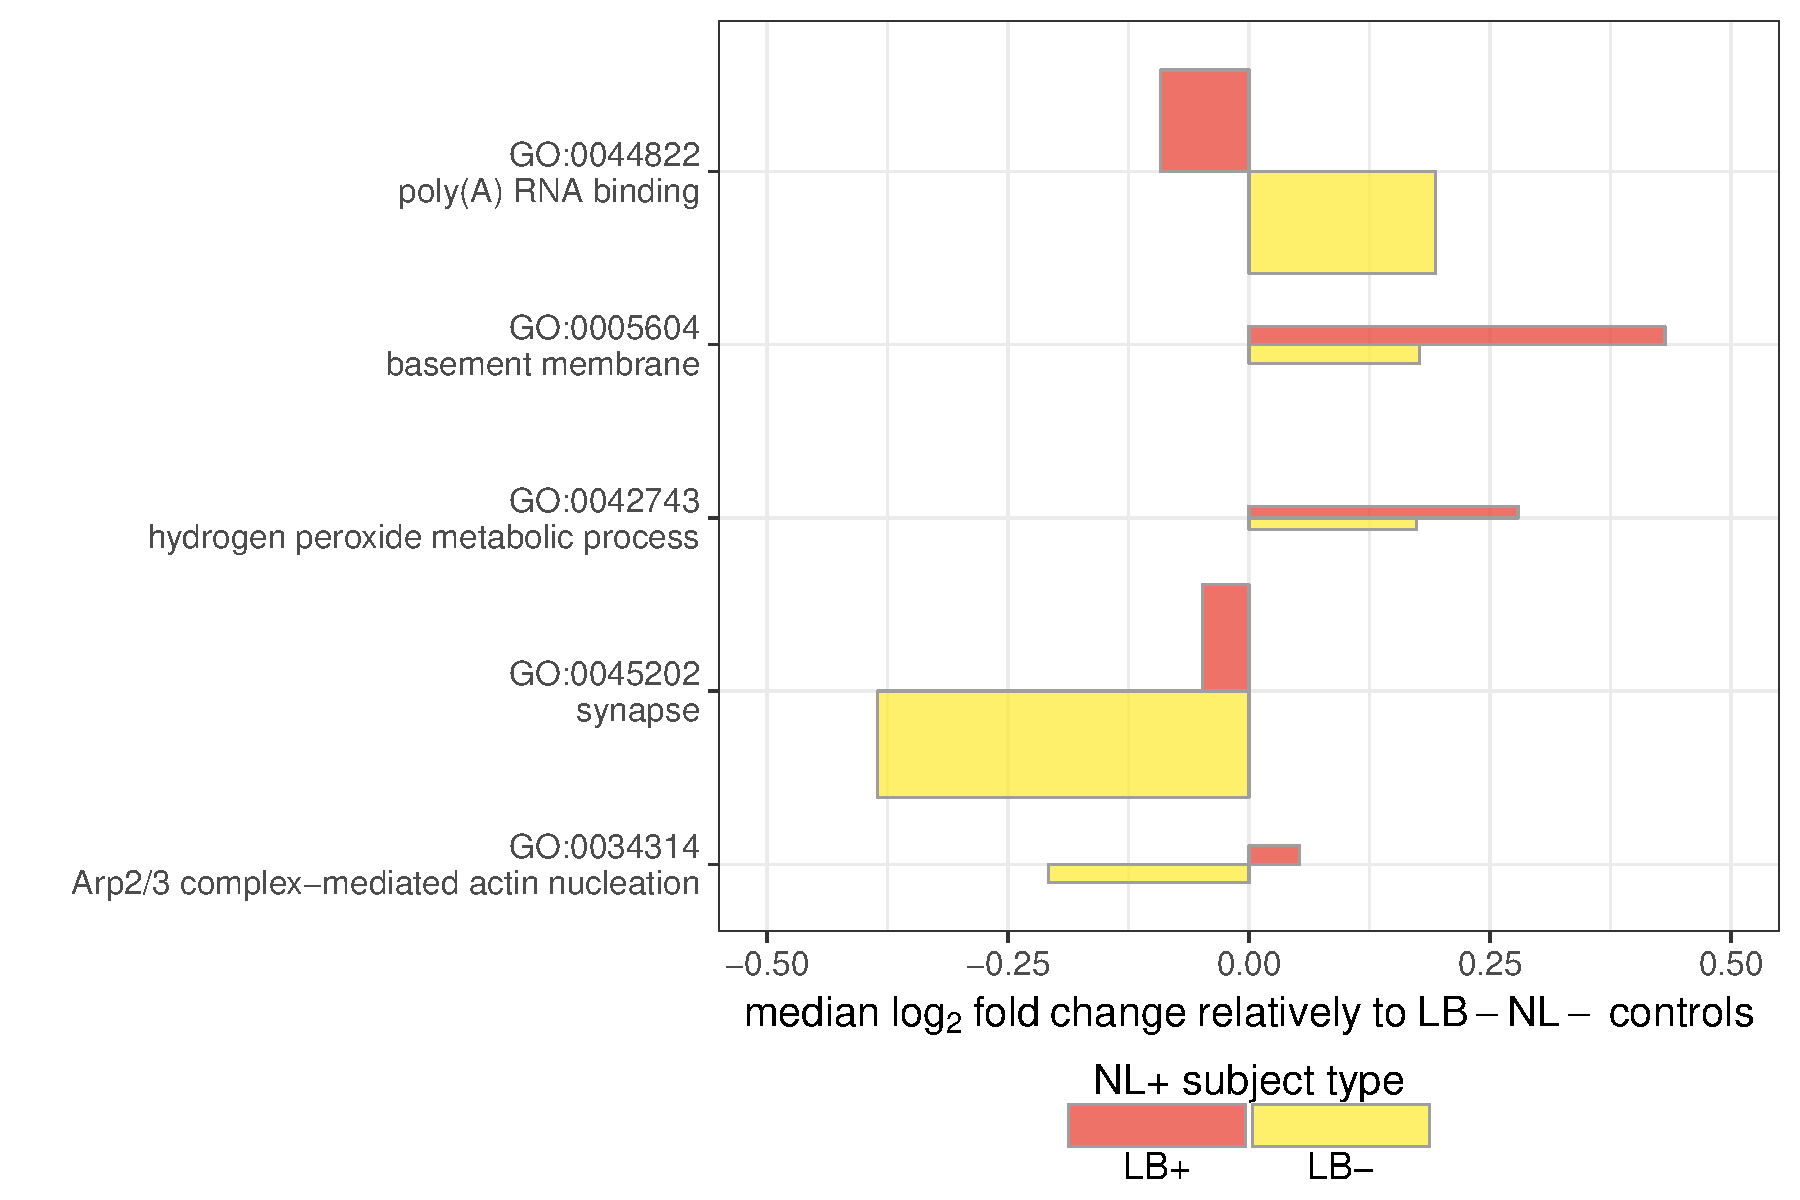
\includegraphics[width=0.99\textwidth]{figure/figure5_barplot-1} 

}



\end{knitrout}
\caption{Corresponds to
\textcolor{black}{\colorbox{highlighter}{\textbf{Figure 5}}} in the main text.
% Quantitative profile of non-redundant set of GO ontology terms
% significantly enriched in proteins with differential abundance. The bar width
% is proportional to the number of proteins mapped to a term. X axis correspond
% to a median log2 fold change between case vs control.2 (red) or
% case vs control.1 (yellow) across a particular GO term.
Non-redundant GO terms. X axis correspond to a median log2 fold change of the corresponding proteins. Control group representing general population (LB-NL-) serves as a reference. The rectangle height (Y axis direction) is proportional to the number of proteins mapped to the term.
}
\label{fig:GObar}
\end{minipage}
\end{figure}




\clearpage







\subsubsection{Heatmaps corresponding to individual terms. Figure 6}



% \begin{figure}[h!]
% \center
% \begin{minipage}{0.9\textwidth}
\begin{knitrout}
\definecolor{shadecolor}{rgb}{0.969, 0.969, 0.969}\color{fgcolor}

{\centering 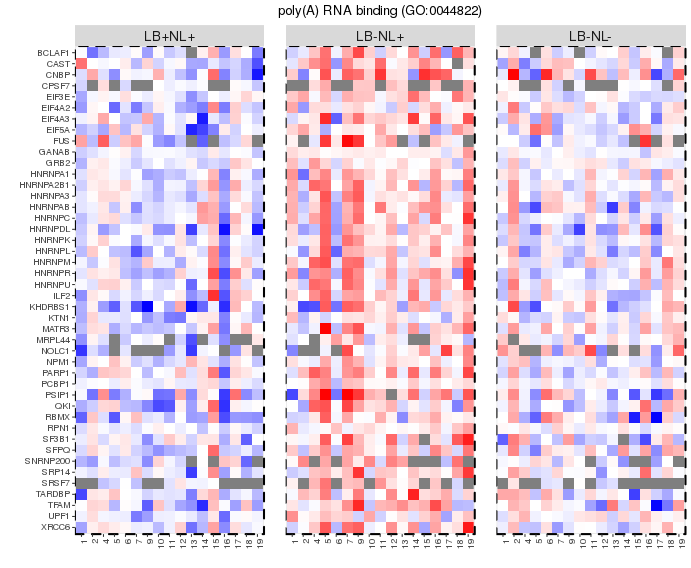
\includegraphics[width=0.75\textwidth]{figure/toppath_heatmaps_5-1} 

}



\end{knitrout}
\begin{knitrout}
\definecolor{shadecolor}{rgb}{0.969, 0.969, 0.969}\color{fgcolor}

{\centering 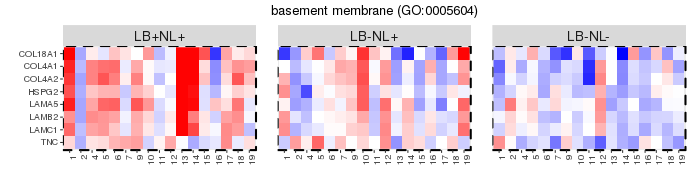
\includegraphics[width=0.75\textwidth]{figure/toppath_heatmaps_4-1} 

}



\end{knitrout}
\begin{knitrout}
\definecolor{shadecolor}{rgb}{0.969, 0.969, 0.969}\color{fgcolor}

{\centering 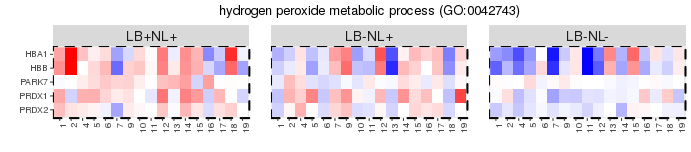
\includegraphics[width=0.75\textwidth]{figure/toppath_heatmaps_3-1} 

}



\end{knitrout}
\begin{knitrout}
\definecolor{shadecolor}{rgb}{0.969, 0.969, 0.969}\color{fgcolor}

{\centering 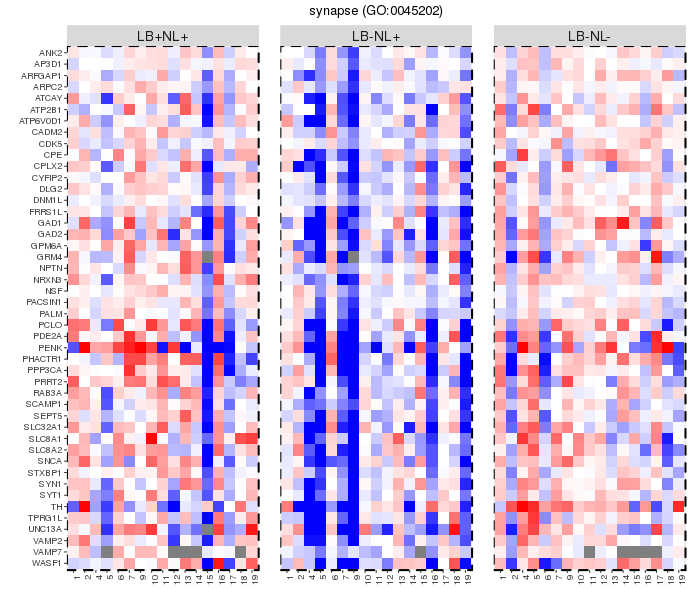
\includegraphics[width=0.75\textwidth]{figure/toppath_heatmaps_2-1} 

}



\end{knitrout}
\begin{knitrout}
\definecolor{shadecolor}{rgb}{0.969, 0.969, 0.969}\color{fgcolor}

{\centering 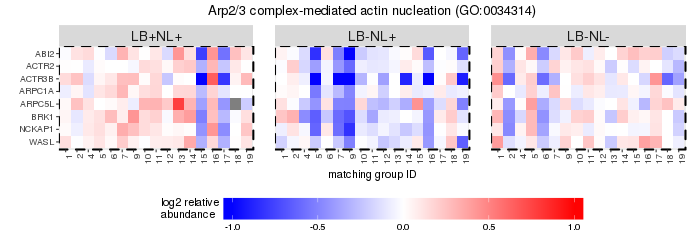
\includegraphics[width=0.75\textwidth]{figure/toppath_heatmaps_1-1} 

}



\end{knitrout}
% \caption{
Corresponds to
\textcolor{black}{\colorbox{highlighter}{\textbf{Figure 6}}} in the main text.
Relative abundances of the individual proteins mapping to the non-redundant 
significant GO terms.
% }
% \label{fig:GOTermsHeatmaps}
% \end{minipage}
% \end{figure}



\clearpage


% part 3



\section{Assessment of the cell type level changes}

The data on cell-specific gene expression was downloaded from 
\href{http://web.stanford.edu/group/barres_lab/brain_rnaseq.html}{Barres Lab}.
Specifically, the excel file with processed data is available
\href{http://web.stanford.edu/group/barres_lab/barreslab_rnaseq.xlsx}{here}.
The corresponding text file is available in the package's "extdata" folder.
The mouse genes were mapped to protein orthologues using ENSEMBL database.
% Note, connection to Biomart is not reliable. Therefore, the
% "ens_ref.RData" file will be downloaded to the package "extdata".
% Moreover, the database may change with the next version.









\subsection{Significance analysis}

Statistical test (Kruskal-Wallis) to check if any cell type changes in 
amount across the subject types. 
The p-values are in the legend to the 
\textcolor{black}{\colorbox{highlighter}{\textbf{Figure 7}}} in the main text. 
Given the data, the endothelial cells are the most strongly associated 
with the neuronal loss regardless of the Lewy bodies.

% latex table generated in R 3.3.2 by xtable 1.8-2 package
% Fri May  8 00:21:09 2020
\begin{table}[ht]
\centering
\begin{tabular}{rrrrrr}
  \hline
 & Astrocyte & Endothelial & Microglia & Neuron & Oligodendrocyte \\ 
  \hline
p-value & 0.071 & 0.0052 & 0.87 & 0.022 & 0.22 \\ 
   \hline
\end{tabular}
\end{table}


\subsection{Barplot of cell type contributions. Figure 7}

\begin{figure}[h!]
\center
\begin{minipage}{0.8\textwidth}
\begin{knitrout}
\definecolor{shadecolor}{rgb}{0.969, 0.969, 0.969}\color{fgcolor}

{\centering 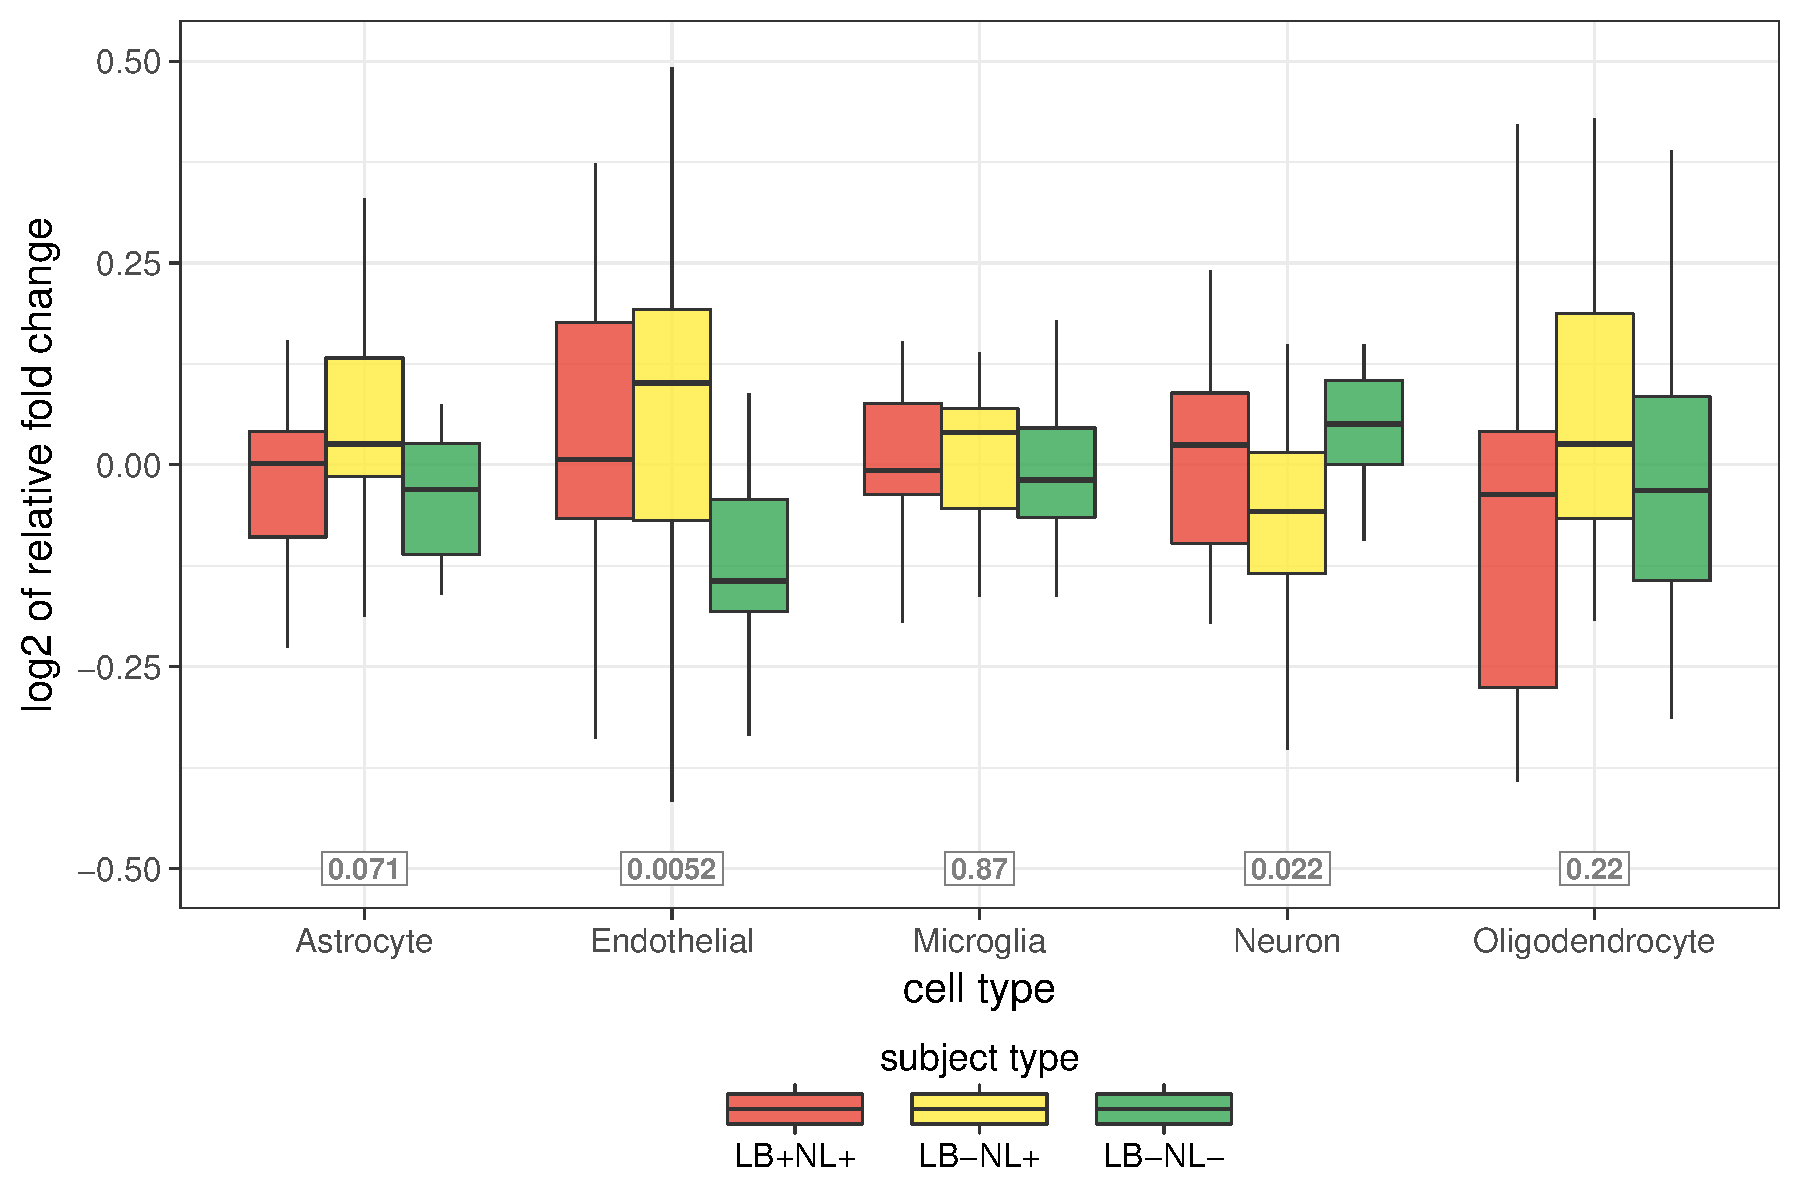
\includegraphics[width=1\textwidth]{figure/cell_type_changes-1} 

}



\end{knitrout}
\caption{Corresponds to
\textcolor{black}{\colorbox{highlighter}{\textbf{Figure 7}}} in the main text.
Estimates of cell-type level changes based on the sets of marker proteins.
Gross cell-level changes were estimated based on the median relative abundance
value of the marker protein sets.}
\label{fig:CellTypes}
\end{minipage}
\end{figure}



\clearpage
\subsection{Heatmap of protein markers of endothelial cells. Figure 8}

\begin{figure}[h!]
\center
\begin{minipage}{1.0\textwidth}
\begin{knitrout}
\definecolor{shadecolor}{rgb}{0.969, 0.969, 0.969}\color{fgcolor}

{\centering 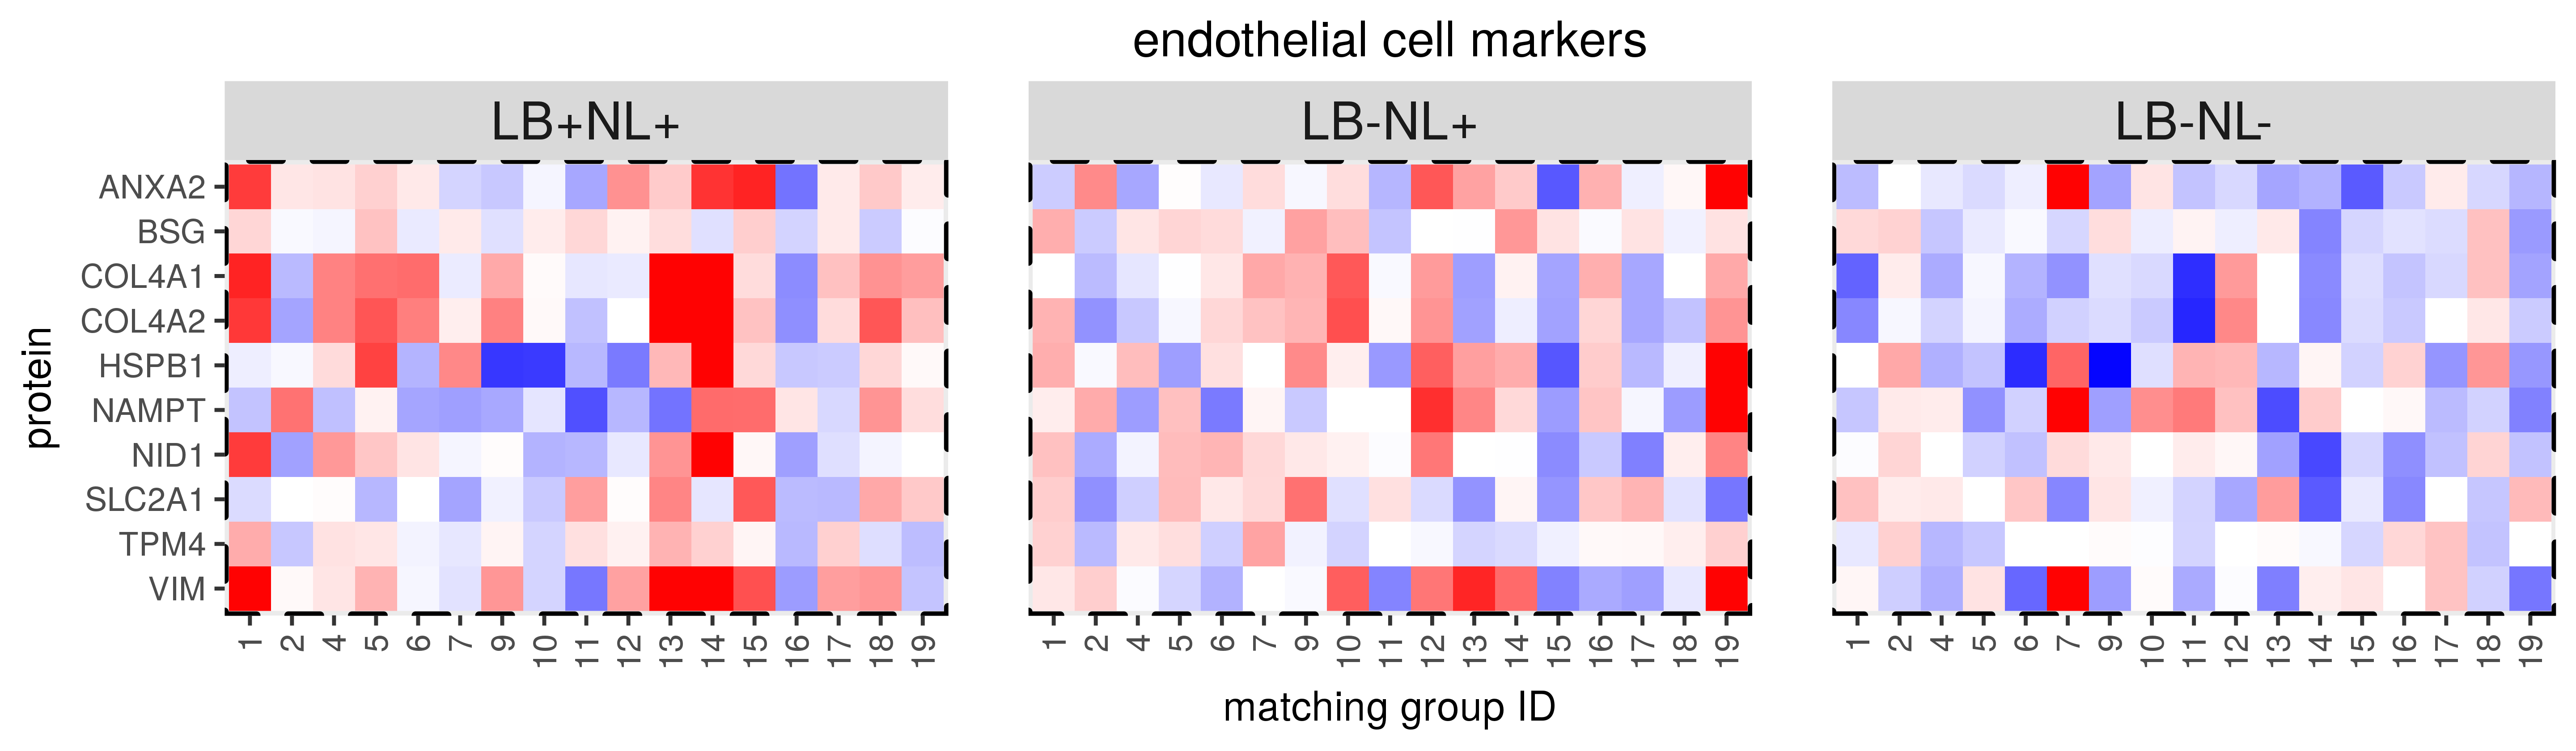
\includegraphics[width=1\textwidth]{figure/endothelial_heatmap-1} 

}



\end{knitrout}
\caption{Corresponds to
\textcolor{black}{\colorbox{highlighter}{\textbf{Figure 8}}} in the main text.
Relative abundances of the endothelial marker proteins. 
The colorkey of relative abundances is the same as on Figure 6.}
\label{fig:EndothelialHeatmaps}
\end{minipage}
\end{figure}

\clearpage





\section{Primary factors affecting $\alpha$-synuclein abundance}

\subsection{Statisical model of $\alpha$-synuclein abundance}

Modeling $\alpha$-synuclein abundance. The terms to consider are the presense of
Lewy bodies (term LB), dopaminergic neuronal loss (term pigmented\_NL) assessed by melanin
deposits and overal neronal cell relative amount estimated using neuronal 
protein markers (term neuron). The random effect terms included plate column and 
matching group. The full model in Wilkinson-Rogers notation is:
\begin{center}
$SNCA \sim LB + pigmented\_NL + neuron + (1|PlateCol) + (1|match.group)$
\end{center}

% latex table generated in R 3.3.2 by xtable 1.8-2 package
% Fri May  8 00:21:13 2020
\begin{table}[ht]
\centering
\begin{tabular}{rlrr}
  \hline
 & term description & p-value & effect size (log2) \\ 
  \hline
LB & Lewy body presence & 0.017 & 0.28 \\ 
  pigmented\_NL & DA neuronal loss & 0.027 & -0.18 \\ 
  neuron & relative amount of neuronal cells & 1.3e-05 & 1.77 \\ 
   \hline
\end{tabular}
\caption{{\color{darkgray} Relation of $\alpha$-synuclein abundance 
and neuropathological parameters.}} 
\end{table}


The results of the statistical modeling indicate that the LB presense 
explain the SNCA abundance. However, given the data, the most strongest
term correlating with SNCA is the amount of neuronal cells.




\section{Causal Network Analysis}







\clearpage

\subsection{Causal Network. Figure 9}
\begin{figure}[h!]
\center
\begin{minipage}{0.95\textwidth}
\begin{knitrout}
\definecolor{shadecolor}{rgb}{0.969, 0.969, 0.969}\color{fgcolor}

{\centering 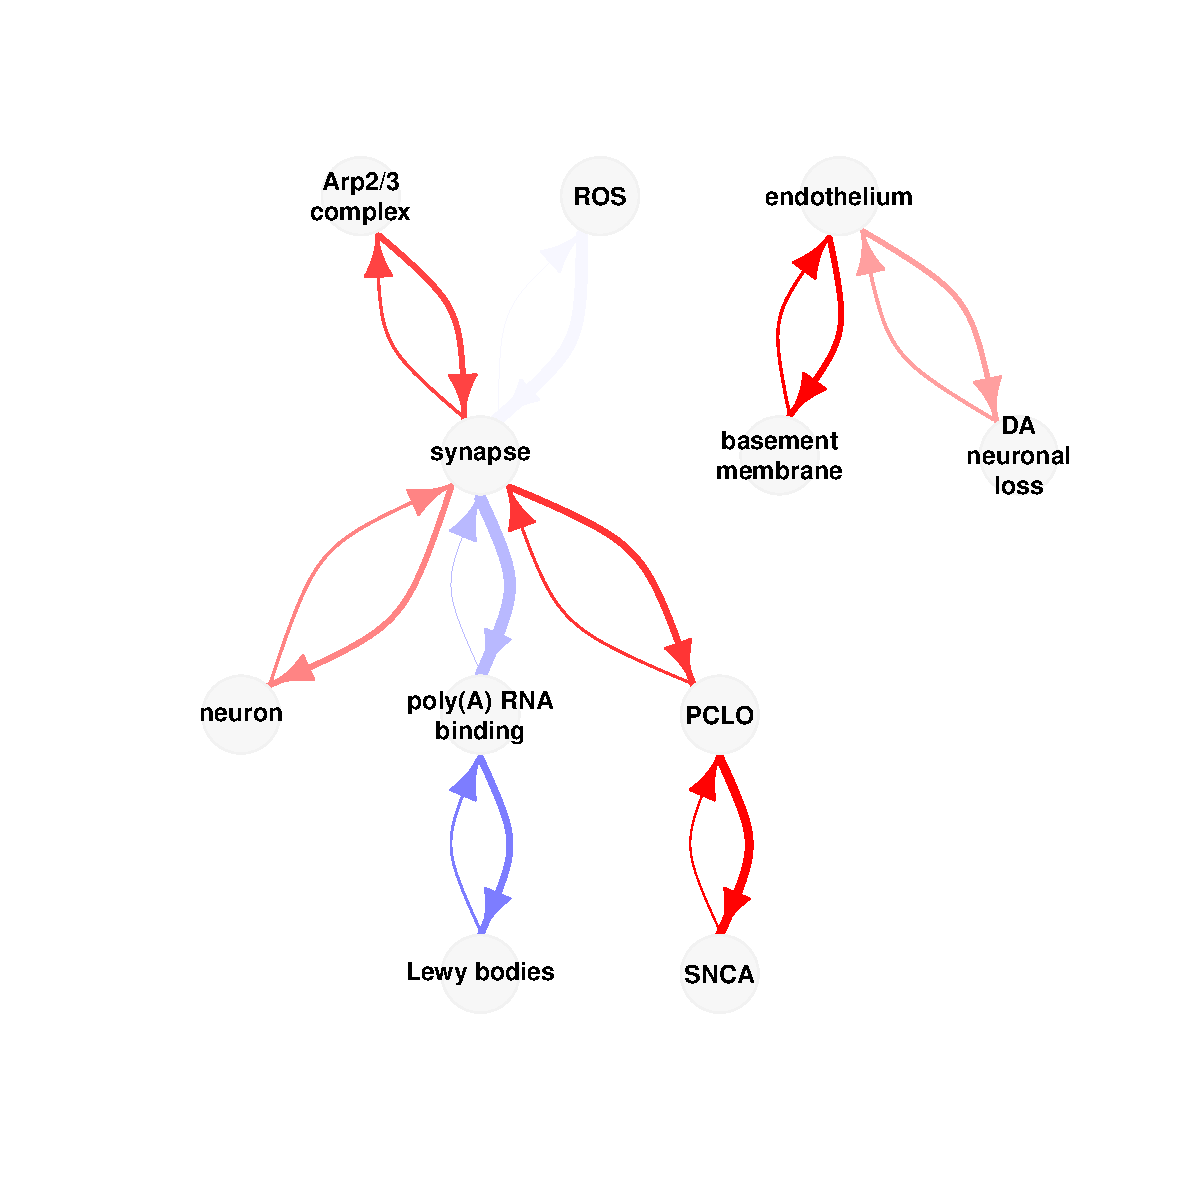
\includegraphics[width=1\textwidth]{figure/visualization_path_causal_network-1} 

}



\end{knitrout}
\caption{Corresponds to \textcolor{black}{\colorbox{highlighter}{\textbf{Figure 9}}} in the main text.
The representation of the causal model and associated uncertainties inferred by
bootstrap analysis. Certainty in edge presence is denoted by opaqueness 
(opaque - more likely). Edge color represents directionality of the effect 
(red - positive, blue -  negative). Confidence in directionality is depicted by 
the edge width. Given the data, the structural modeling does not suggest 
$\alpha$-synuclein as the major driver of LB formation.}
\label{fig:CausalPathNetwork}
\end{minipage}
\end{figure}





\clearpage
\section{Session information}
All software and respective versions used in this document, as returned by sessionInfo() are detailed below.
\small
\begin{itemize}\raggedright
  \item R version 3.3.2 (2016-10-31), \verb|x86_64-pc-linux-gnu|
  \item Locale: \verb|LC_CTYPE=en_US.UTF-8|, \verb|LC_NUMERIC=C|, \verb|LC_TIME=en_US.UTF-8|, \verb|LC_COLLATE=en_US.UTF-8|, \verb|LC_MONETARY=en_US.UTF-8|, \verb|LC_MESSAGES=C|, \verb|LC_PAPER=en_US.UTF-8|, \verb|LC_NAME=C|, \verb|LC_ADDRESS=C|, \verb|LC_TELEPHONE=C|, \verb|LC_MEASUREMENT=en_US.UTF-8|, \verb|LC_IDENTIFICATION=C|
  \item Base packages: base, datasets, graphics, grDevices, grid, methods,
    parallel, stats, stats4, utils
  \item Other packages: AnnotationDbi~1.36.2, Biobase~2.34.0,
    BiocGenerics~0.20.0, BiocParallel~1.8.2, BiocStyle~2.2.1, bnlearn~4.0,
    Category~2.40.0, clusterProfiler~3.2.14, doParallel~1.0.10, DOSE~3.0.10,
    dplyr~0.5.0, dynamicTreeCut~1.63-1, fastcluster~1.1.20, foreach~1.4.3,
    gelnet~1.2.1, ggbeeswarm~0.5.0, ggplot2~2.2.1, GOstats~2.40.0, graph~1.52.0,
    igraph~1.0.1, IRanges~2.8.2, iterators~1.0.8, knitr~1.14, lme4~1.1-12,
    lubridate~1.6.0, MASS~7.3-45, Matrix~1.2-7.1, MSnbase~2.0.2, multcomp~1.4-5,
    mvtnorm~1.0-6, mzR~2.8.1, org.Hs.eg.db~3.4.0, pcaMethods~1.66.0,
    ProtGenerics~1.6.0, qvalue~2.6.0, Rcpp~0.12.9, ReactomePA~1.18.1,
    reshape2~1.4.1, S4Vectors~0.12.2, survival~2.40-1, TH.data~1.0-8,
    tidyr~0.6.1, vp.misc~0.1, WGCNA~1.51, xtable~1.8-2
  \item Loaded via a namespace (and not attached): acepack~1.4.1, ade4~1.7-4,
    affy~1.52.0, affyio~1.44.0, annotate~1.52.1, AnnotationForge~1.16.1,
    assertthat~0.1, backports~1.0.5, base64enc~0.1-3, beeswarm~0.2.3,
    BiocInstaller~1.24.0, bitops~1.0-6, Boruta~5.0.0, caTools~1.17.1,
    checkmate~1.8.2, cluster~2.0.5, codetools~0.2-15, colorspace~1.3-2,
    data.table~1.10.4, DBI~0.5-1, digest~0.6.9, DO.db~2.9, evaluate~0.10,
    fastmatch~1.0-4, FField~0.1.0, fgsea~1.0.2, foreign~0.8-67, formatR~1.4,
    Formula~1.2-1, gdata~2.17.0, genefilter~1.56.0, glmnet~2.0-5, GO.db~3.4.0,
    GOSemSim~2.0.4, gplots~3.0.1, graphite~1.20.1, gridExtra~2.2.1,
    GSEABase~1.36.0, gtable~0.2.0, gtools~3.5.0, Hmisc~4.0-2, htmlTable~1.9,
    htmltools~0.3.5, htmlwidgets~0.8, impute~1.48.0, KernSmooth~2.23-15,
    labeling~0.3, lattice~0.20-34, latticeExtra~0.6-28, lazyeval~0.2.0,
    limma~3.30.13, magrittr~1.5, MALDIquant~1.14, matrixStats~0.50.2,
    memoise~1.0.0, minqa~1.2.4, munsell~0.4.3, mzID~1.12.0, nlme~3.1-128,
    nloptr~1.0.4, nnet~7.3-12, outliers~0.14, plyr~1.8.4, preprocessCore~1.36.0,
    R6~2.2.0, randomForest~4.6-12, ranger~0.4.0, rappdirs~0.3.1, RBGL~1.50.0,
    RColorBrewer~1.1-2, RCurl~1.95-4.8, reactome.db~1.58.0, Rgraphviz~2.18.0,
    ROCR~1.0-7, rpart~4.1-10, RSQLite~1.1-2, sandwich~2.3-4, scales~0.4.1,
    splines~3.3.2, stringi~1.1.2, stringr~1.2.0, tibble~1.2, tools~3.3.2,
    varSelRF~0.7-5, vipor~0.3.2, vsn~3.42.3, XML~3.98-1.5, zlibbioc~1.20.0,
    zoo~1.7-14
\end{itemize}


\end{document}





